\chapter{Experiments and Lab Work}\label{ch:experiment}
To relate the theory behind controlling pumps to the real world,
we conducted different experiments.

System tests were carried out to gather data about how the system reacts under different conditions.
The measured data was stored for further analysis.
From the data it was possible to identify the correlations between pump speed, 
backpressure, flow and power consumption. 
The data also makes it possible to extrapolate equations for the system,
that estimates the systems reaction at different conditions.

The actual tests were performed by running a pump at different speed intervals,
while varying the flow resistance by the control valve.
This results in corresponding values of flow, pressure, and energy consumption
measured by the sensors.

\section{Data Acquisition}\label{sec:data_gathering}
The pump system is built as described in Chapter \ref{ch:physsetup},
with the controlling PC running xPC Target,
a real-time OS for use with SLRT. 

All data was collected with the help of custom made 
ML scripts and SLRT models.
The execution of these was done on the xPC Target OS.
Specific parts of these files will be explained in this chapter,
while the complete files can be found on the GitHub repository \cite{GitHub}.

To use SLRT on xPC targets, a SL model of the system was made on the host PC,
compiled, transferred over Ethernet and executed on the xPC target.
After the real-time execution is finished on the target,
the .dat files containing the recorded data have to be transferred back to the host,
where further analysis can be done.

To automate as much of this process as possible,
we created a ML script that updates and compiles the SL model, transfers it to the target,
starts the execution and copies the generated .dat files to the host.

\section{System Test}\label{sec:system_test} 
It was expected that the controller would change the the pump speed $\omega P_{1,2,3}$,
we decided to fix the backpressure by fixing the control valve position,
and stepwise change $\omega P_{1,2,3}$.
Since the three pumps in the setup are expected to be identical,
the test was only run with one of the pumps.

To get reliable results, we chose to only change one variable at a time.

The pump speed was gradually changed in order to monitor the flow, pressure and power consumption.
Starting from 0\% pump speed, we have increased the speed by 10\% every 15 seconds. This was done
in order to give the system some time to stabilize. The process was repeated for a range of valve openings.
Identical to the pump speed, the valve was in the beginning 10\% open, gradually increasing by 10\% and
finally reaching 100\%.
Several identical tests were conducted, in order to see if the values would hold.

Figure \ref{fig:measuredFlow} represents the flow, while Figure \ref{fig:measuredPower}
and Figure represent the pressure and power consumption, respectively.

\begin{figure}[ht]
	\centering
	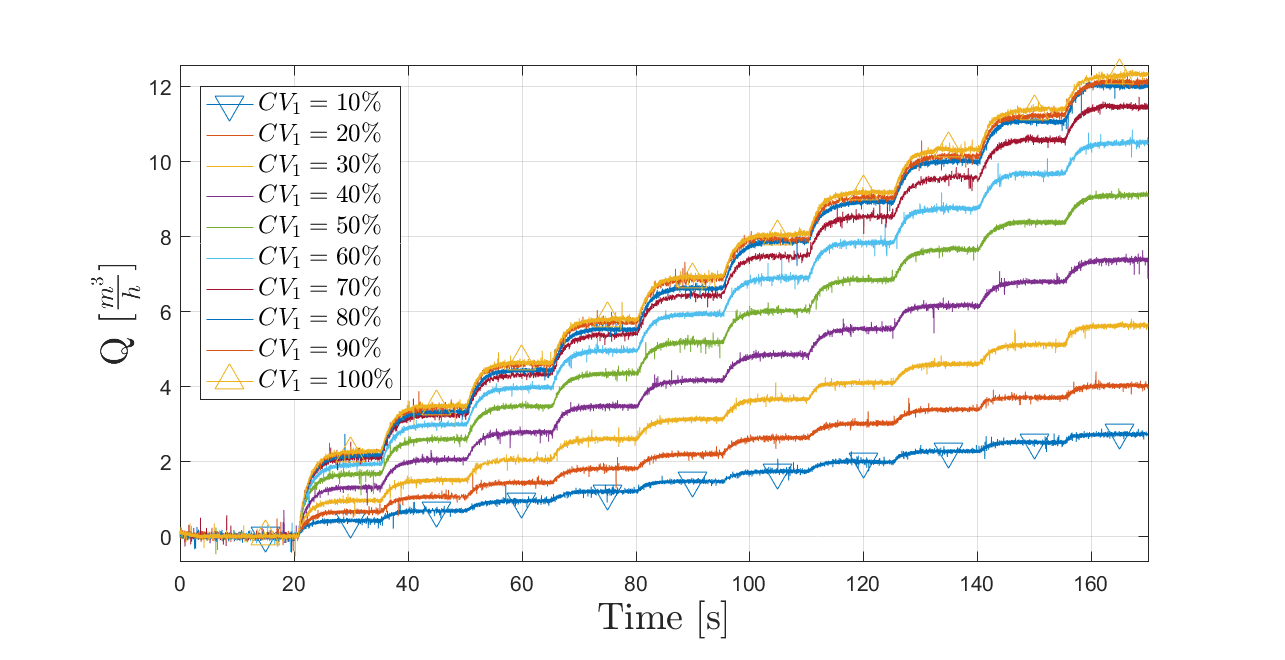
\includegraphics[scale=0.5]{figures/05mathematicalModelling/measuredFlow.eps}
	\vspace{-5mm}
	\caption{Measured Flow}
	\label{fig:measuredFlow}
\end{figure}
\vspace{-5mm}
\begin{figure}[ht]
	\centering
	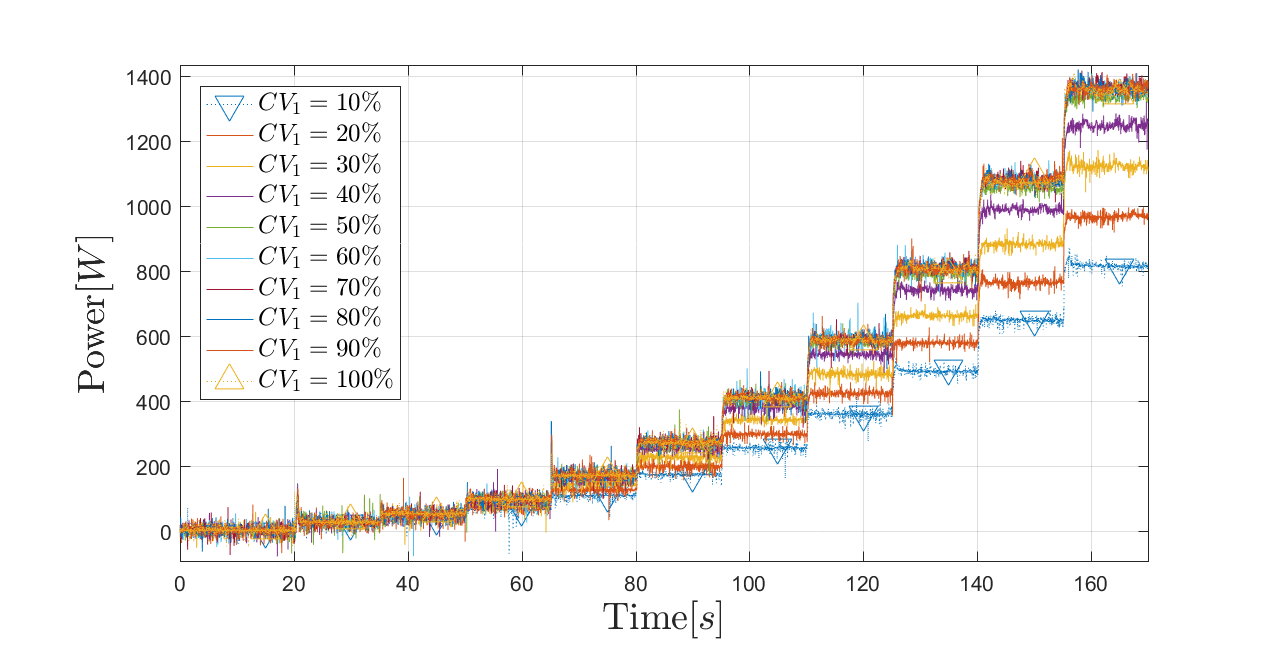
\includegraphics[width=0.81\textwidth]{figures/05mathematicalModelling/measuredPower.eps}
	\vspace{-5mm}
	\caption{Measured Power}
	\label{fig:measuredPower}
\end{figure}

\todo[color=04mathematicalModelling]{fix formatting later and also add for pressure}

\section{Data Example}\label{sec:results}
A system test was performed, 
to capture live data of how the system would react, 
under various conditions.
The pump speed was gradually turned up from 0 to 100\% in intervals of 10\%. 
During each pump speed, the control valve was changed in 10\% intervals as well. 
For each change to the control valve, 
10 seconds of settling time was introduced, 
to let the control valve and backpressure stabilise.

Figure X shows the captured data for a test, with pump at 50\% speed and control valve at 50\%.

\begin{figure}[ht]
	\centering
	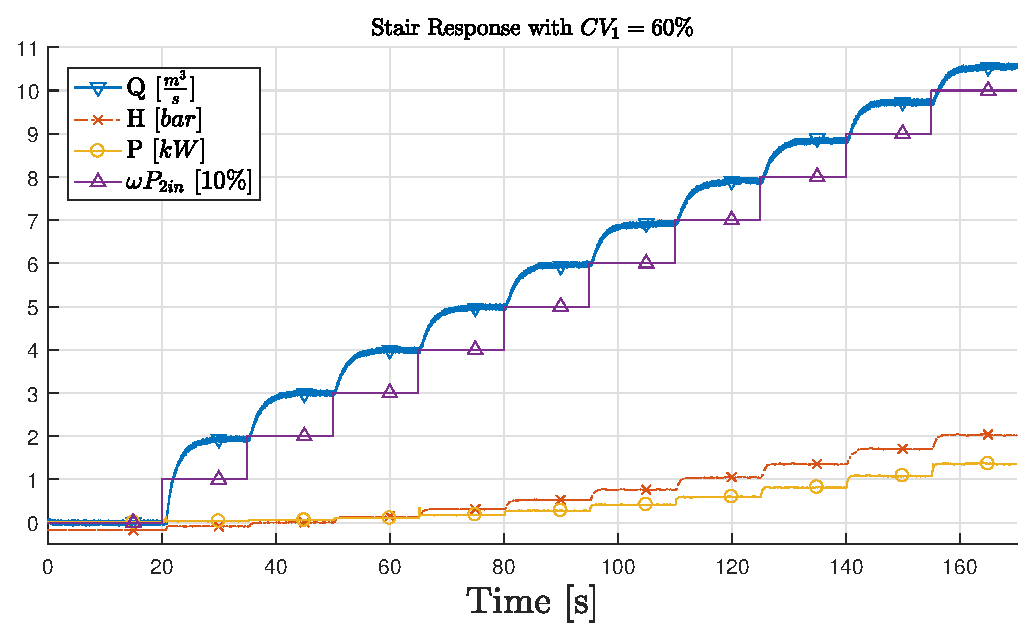
\includegraphics[width=0.8\textwidth]{figures/04ExperimentsAndLabWork/testrun}
	\vspace{-5mm}
	\caption{testrun}
	\label{fig:testrun}
\end{figure}
%Show curves from early test runs